\documentclass[9pt]{article}
\usepackage{geometry}
\geometry{a4paper}
\usepackage{graphicx}
\usepackage{hyperref}
\usepackage{float}
\usepackage{wrapfig}
\usepackage{csquotes}
\linespread{1.2}
\graphicspath{{Pictures/}}

\begin{document}

%----------------------------------------------------------------------------------------
%	TITLE PAGE
%----------------------------------------------------------------------------------------

\begin{titlepage}

\newcommand{\HRule}{\rule{\linewidth}{0.5mm}}
\center
\textsc{\LARGE University of Southampton}\\[1.5cm]
\textsc{\Large Msc Cyber Security}\\[0.5cm]
\textsc{\large Foundation of Cyber Security}\\[0.5cm]
\HRule \\[0.4cm]
{ \huge \bfseries Privacy Laws}\\[0.4cm]
\HRule \\[1.5cm]

\begin{minipage}{0.4\textwidth}
\begin{flushleft} \large
\emph{Author:}\\
Gerard \textsc{Tio Nogueras}
\end{flushleft}
\end{minipage}
~
\begin{minipage}{0.4\textwidth}
\begin{flushright} \large
\emph{Supervisor:} \\
Pr. Vladimiro \textsc{Sassone}
\end{flushright}
\end{minipage}\\[4cm]

{\large \today}\\[3cm]
%\includegraphics{Logo}\\[1cm] % Include a department/university logo - this will require the graphicx package

\vfill
\end{titlepage}
%----------------------------------------------------------------------------------------
%	INTRODUCTION
%----------------------------------------------------------------------------------------

\section{Introduction}
In 2016 the data protection laws are still being modified to keep up with the growth of IoT, Big Data and the general expansion of internet. There are a couple of important definitions concerning the scope of the Data Protection Act that still raise debate and we will present these heated topics and discuss them.\\
We have two questions to introduce them:
\begin{enumerate}
\item Simply put, it is not possible to de-identify individual personal data unless you are talking about a single, low resolution measurement in total isolation.\\
\textbf{Critically discuss the above statement by assessing what the implications of such a statement would be for law-makers wanting to better delineate the domain of data protection laws.}
\item WP29: A specific  pitfall  is  to consider pseudonymised  data  to  be  equivalent to anonymised data. ICO:  Pseudonymisation is a way to produce anonymised data but on an individual-level basis\\
\textbf{Are these statements inconsistent? Critically discuss with references to both documents. }
\end{enumerate}
%----------------------------------------------------------------------------------------
%	CONTENT
%----------------------------------------------------------------------------------------

\section{Content}
\subsection{1st Part}

\subsubsection{Understanding the statements and explaining the state of the art of privacy laws}
Let us try to understand the first statement by analysing its different parts and discussing some definitions. We will use different sources to define sensitive words and the first one is \textbf{de-identify}:\\\\
The \textbf{ICO} (Information Commissioner's Office) is the office responsible for the enforcement of the Data Protection Act 1998(DPA) which \enquote{principles of protection must apply to any information concerning an identified or identifiable person.}\cite{ICO:PD}\\
The \textbf{CJEU} Court of Justice of the European Union) enforces the \textbf{DPD} (Data Protection Directive) 95/46/EC. They do not provide a direct definition of de-identification but instead they define identifiable: \enquote{To determine whether a person is identifiable, account should be taken of all the means likely reasonably to be used either by the controller or by any other person to identify the said person.} \cite{CJEU - DPD 1995}\\
The \textbf{GDPR} (General Data Protection Regulation) is the new regulation that will replace the DPD in 2018. Their definition is very similar to the DPD:\enquote{To determine whether a person is identifiable, account should be taken of all the means reasonably likely to be used, such as singling out, either by the controller or by any other person to identify the individual directly or indirectly.}\cite{GDPR:2016}\\\\
The second word that is worth our attention is \textbf{personal data}, here we will aim for less quantity and more quality meaning that we will try to bring the ones with different visions. \\
The interest for this word is that \enquote{ICO enforces the DPA and the DPA stipulates that it only applies to personal data} this starts a debate to clearly define what is considered personal data with regards of its processing and its free movement. We will first understand what is considered personal data then discuss the scope that it represents.\\\\
The DPD defines personal data as \enquote{any information relating to an identified or identifiable natural person}\cite{CJEU - DPD 1995} then goes on and defines identifiable person: \enquote{one who can be identified, directly or indirectly, in particular by reference to an identification number or to one or more factors specific to his physical, physiological, mental, economic, cultural or social identity.} \cite{CJEU - DPD 1995}\\ The GDPR has the same definition concerning personal data but has an updated definition concerning an identifiable person \enquote{one who can be identified directly or indirectly, in particular by reference to an identifier such as a name, an identification number, location data, online identifier or to one or more factors specific to the physical, physiological, genetic, mental, economic, cultural or social identity of that person.} \cite{DPD-GDPR:1995-2018}\\We realize with those definitions that the interesting part is actually knowing what is considered an identifiable person which will be one of the subjects discussed further below.\\ The Working Party has given its opinion of this part of the directive "to determine ... the said person"\cite{CJEU - DPD 1995}. The Directive suggested it as a criterion to be applied in order to assess whether the anonymisation  process is sufficiently robust.\cite{WP29:2007} WP Art.29 argued that the particular context and circumstances of a specific case directly impact on identifiability. \cite{Sophie:2016}\\\\To sum up the statement, they(law entities) are trying to identify what to perceive and consider as personal data and the ability to be rendered it unlinkable to the data subjects (Data subject means an individual who is the subject of personal data).

\subsubsection{Implications of these statements} 

The implications are straightforward, the definition of \textbf{personal data} is the centre of the discussion, followed by \textbf{identifiable person} which is included in personal data and finally which will be discussed in the second question, when can data no longer be considered personal data and therefore be outside the scope of the DPA.(\textbf{de-intendified})\\
If you consider the initial statement, the consequences would be that single, low resolution measurements in total isolation would fall off the DPA scope and therefore would not be restricted anymore. This could be used by any data processor/controller to try and escape regulations by abusing this exception and hiding behind it if sued.
\subsubsection{Discussion of these implications and critical assessment of the different arguments}
We will start the discussion by talking of one of the most waited decisions this year concerning personal data, which is the Case of Breyer v Germany.
With the final decision on the Breyer Case that got released 19 October 2016 what are the consequences?\cite{IP:10}\\
\enquote{The CJEU essentially decided that dynamic IP addresses collected by an online media service provider only constitute personal data if the possibility to combine the address with data necessary to identify the user of a website held by a third party (...) constitutes a mean \enquote{likely reasonably to be used to identify} the individual.}\\
The court basically stated: \enquote{that it is not sufficient that only a third party may identify the individual with the data it holds that additional data that is held by third parties necessary to identify an individual is in relation to a party only relevant if the possibility to combine this data constitutes a means likely reasonably to be used to identify the individual which requires that the identification of the data subject must be legally and practically possible for that party}\cite{Breyer:2016}\\ It seems that the final answer is still \enquote{\textbf{IT DEPENDS}} since data still has to be approached on a case-to-case basis. If IP addresses were considered personal data \enquote{data controllers and processors would have to treat IP addresses in accordance with the Directive’s stringent data handling requirements.} Later on they mention the practical implications: \enquote{Defining dynamic IP addresses as personal data therefore would impose fairly stringent restrictions on the processing of that information.  Companies that seek to identify users through their IP addresses – whether for tracking, marketing, or other purposes – therefore should take note of the continuing developments in this area.} \cite{Proskauer}\\
\\
As shown in the definitions, the GDPR has upgraded its scope of identifiers which shows its goal to keep up with its time. With new researches and technologies those had to be taken in account( genetic data, biometric data, location data, online identifiers). Nonetheless, some are missing from the list: \enquote{IP addresses, MAC addresses and other identifiers are not explicitly mentioned in the Directive.}\cite{DPD-GDPR:1995-2018}. We can see that there is still some progress, we know that these identifiers are not easy to add to the list due to their major global use and probably a lot of research and agreements will be needed before they can be added.\\
\\
Another good thing that the WP29 pointed out was the fact that the de-identification of certain data has to be made knowing who is going to use them and for what goal that way you can target the de-identification specifically to the case. This is the only way you will make sure to provide the higher chances of privacy to the data subjects. There a lot of techniques used to achieve this de-identification, more details on these will be discussed in the second question.\cite{differential privacy}\cite{WP29:2007}\cite{Sophie:2016}\\
\\
This last point is for me the most important and the strongest argument, de-identification and evaluation of personal data on a case-to-case basis is the best option in my opinion, it might not be the most effective but it assures a really strong privacy protection.

\subsection{2nd Part}
\subsubsection{Understanding the statements}
The statement simply opens up the discussion to the strength and use of pseudonymisation and should it be considered anonymisation on an individual basis. Let us state the different views from both parties. For the ICO, anonymisation: \enquote{Anonymisation is the process of turning data into a form which does not identify individuals and where identification is not likely to take place.} and pseudonymisation: \enquote{anonymised data but on an individual-level basis}\cite{Anonymisation(ICO)}
and for the WP29, anonymization: \enquote{transforming personal information into data that can no longer be used to identify a natural person taking into account all the means likely reasonably to be used by either the controller or a third party.  An important factor is that the processing must be irreversible.} and pseudonymisation: \enquote{A  specific  pitfall  is  to consider pseudonymised  data  to be  equivalent  to anonymised  data}
It is important to say that the WP29 has reserves to anonymization: \enquote{it is critical to understand  that  when a data controller does not delete the original  (identifiable) data at event-level, and the data controller hands over part of this dataset (for example after removal or masking of identifiable data), the  resulting dataset is still personal data!} and \cite{Pseudonymisation}\cite{WP29:2007}
\subsubsection{Implications and Discussion of these statements}
Like said in the ICO code of practice \cite{code of practice} the centre of everything is the definition of personal data for this refer to the previous question to have a clear definition. 
The reason for that is the DPD makes it clear that \enquote{the principles of data protection shall not apply to data rendered anonymous in such a way that the data subject is no longer identifiable.}\cite{CJEU - DPD 1995} similarly the WP29: \enquote{Once a dataset is truly anonymised and individuals are no longer identifiable, European data protection law no longer applies}. So the effect from this ruling should be that all data controllers anonymise their data but it is not, instead many opt to pseudonymize it instead. Here are some of the reasons: \enquote{strength of pseudonymisation undervalued and sufficient for individual expectations, impossibility of anonymisation regarding the business model of certain companies which is based on individual records, need for reversibility (clinical trials) and improvement of the security for data controllers in data breach scenarios.}\cite{Pseudonymisation}\\\\
What is the opinion of the GDPR about the matter: The key distinction between pseudonymised data, which is regulated and anonymous data, which is not, is whether the data can be re-identified with reasonable effort.\cite{GDPR:2016}
The GDPR considers pseudonymization as a means of protecting the rights of individuals while also allowing controllers to benefit from the data’s utility. Even if pseudonymized data still falls within its scope some provisions are relaxed to encourage controllers to use the technique. Thus, controllers will have an easier time using personal data for secondary purposes and for scientific research. It is important to raise awareness around a contradiction introduced in the GDPR which should reviewed: the definition of pseudonymisation in Art. 4 and the statement introduced in recital 26 which equates pseudonymised data to personal data.\cite{Sophie:2016}\cite{GDPR:2014}\\\\
NIST opinion: they acknowledge that de-identification tries its best to keep personal data from being identifiable knowing to some extent this isn't achievable to perfection.\cite{NIST:2015} \\
In the NIST report: \enquote{Anonymization is another subcategory of de-identification. Unlike pseudonymization, it does not provide a means by which the information may be linked to the same person across multiple data records or information systems. Hence, re-identification of anonymized data is not possible.}\cite{NIST:2015} This definition is really close to the one stated by the WP29. The NIST have good recommendations for de-identification that follow the stream of the technical ideas discussed by the WP29. They employ 2 techniques, the first is the suppression of 18 identifiers and the second is a statistical approach close to the differential privacy technique. Here is the advices given by the WP29 when choosing a certain process of de-identification.
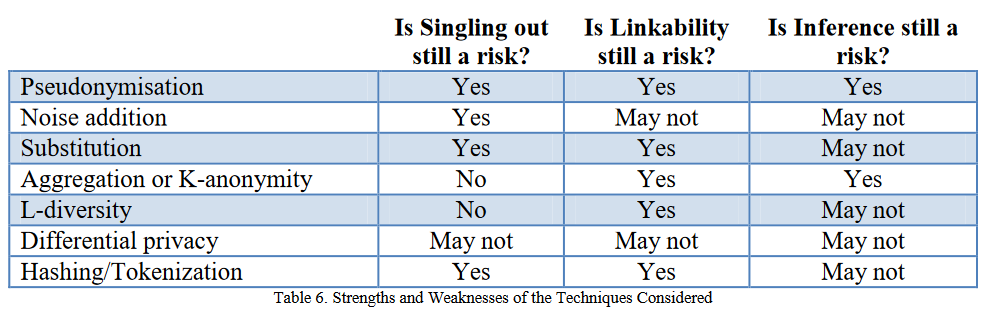
\includegraphics[scale=0.55]{techniques.png}
\cite{WP29:2007}\\\\
The Working Party's opinion on anonymisation: \enquote{Anonymisation is a technique applied to personal data in order to achieve irreversible de-identification.\\
Techniques of de-identification and anonymisation are the subject of intense research each technique has its advantages and disadvantages. In most cases it is not possible to give minimum recommendations for parameters to use as each 
dataset needs to be considered on a case-by-case basis.}\\
The Working Party stresses that \enquote{anonymisation techniques can provide privacy guarantees, but only if their application is engineered appropriately which means that the context and the objectives of the anonymisation process must be clearly set out in order to achieve the targeted anonymisation level.}\cite{WP29:2007}\\\\
The problem with these definitions is that some anonymization attempts have resulted in data being re-identified, implying that the date thought to be anonymized actually weren’t.\cite{ICO:PD}
In many cases, an anonymised dataset can still present residual risk to data subjects. Indeed, even when it is no  longer possible to precisely retrieve the record of an  individual, it may remain possible to glean information about  that individual with the help of other sources of information that are available\cite{WP29:2007}. One of the first big examples of this is the Netflix Prize Dataset\cite{Netflix} which disclosed an anonymised dataset which was re-identified with the combination of a rating dataset from IMDB the Internet Movie database.\\\\
To answer the main question, the answer is no. The reason being that anonymised data does not enter the scope of regulations and pseudonymised data does. Even if the statement of the ICO might be accurate you rarely de-identify a single piece of data, you are usually facing an aggregate in which case the statement is not valid anymore. If it was misunderstood that pseudonymisation was equivalent to anonymization then all the pseudonymised data would be out of the scope of the regulations and this would represent big risks for the data subjects, since all the entities agree that pseudonymisation is a great tool but allows for a high risk of identification.
In my opinion pseudonymisation should always be encouraged as a minimum measure intended to facilitate data use but never considered as anonymised data.\\
And finally can we consider anonymised data to be honest with its definition, unfortunately as all our teachers repeat time and time again, with resources and determination nothing is perfectly secured, same goes here no anonymised dataset is perfectly protected. 

%----------------------------------------------------------------------------------------
%	BIBLIOGRAPHY
%----------------------------------------------------------------------------------------
\newpage
\begin{thebibliography}{99}
\bibitem[NIST,2015]{NIST:2015}L. Garfinke, S. (2015) De - Identi fi cation of Personal Information. Available at: \url{https://www.huntonprivacyblog.com/wp-content/uploads/sites/18/2015/10/NIST.IR_.8053.pdf} (Accessed: 2 November 2016).

\bibitem[Summary of the HIPAA privacy rule (2013)]{HSS:2000}Summary of the HIPAA privacy rule (2013) Available at: \url{http://www.hhs.gov/hipaa/for-professionals/privacy/laws-regulations/index.html} (Accessed: 2 November 2016).

\bibitem[EU Directive 95/46/EC - The Data Protection Directive, 1995]{CJEU - DPD 1995}EU Directive 95/46/EC - The Data Protection Directive (1995) Available at: \url{https://www.dataprotection.ie/docs/EU-Directive-95-46-EC-Chapter-1/92.html} and at \url{http://eur-lex.europa.eu/legal-content/en/TXT/?uri=CELEX%3A31995L0046}(Accessed: 2 November 2016).

\bibitem[European privacy officers forum (EPOF), 2009]{EPOF:2009-2011} European privacy officers forum (EPOF) (2009) Available at: \url{http://www.epof.org/} (Accessed: 2 November 2016).

\bibitem[Maldoff, 2016]{GDPR:2016}Maldoff, G. (2016) Top 10 operational impacts of the GDPR: Part 8 - Pseudonymization. Available at: https://iapp.org/news/a/top-10-operational-impacts-of-the-gdpr-part-8-pseudonymization/ (Accessed: 2 November 2016).

\bibitem[Slaugther and May, 2016]{DPD-GDPR:1995-2018}Personal data, anonymisation and pseudonymisation under the GDPR.(2016)  Available at: https://www.slaughterandmay.com/media/2535637/personal-data-anonymisation-and-pseudonymisation-under-the-gdpr.pdf (Accessed: 2 November 2016).

\bibitem[WP29, 2014]{WP29:2007} ARTICLE 29 DATA PROTECTION WORKING PARTY (2014) Opinion 05 /2014 on Anonymisation Techniques. Available at: \url{http://www.cnpd.public.lu/fr/publications/groupe-art29/wp216_en.pdf} (Accessed: 2 November 2016).

\bibitem[Stalla - Bourdillon, 2016]{Sophie:2016}Stalla - Bourdillon, S. (2016) Cybersecurity and the Law Introduction to Data Protection Law. Available at: \url{https://secure.ecs.soton.ac.uk/noteswiki/images/comp6224%2816%29_02Introductiontodataprotection2.pdf (Accessed: 2 November 2016).}

\bibitem[European Parliament, 2013]{GDPR:2014}The European Parliament (2013) European Parliament legislative resolution of 12 March 2014 on the proposal for a regulation of the European Parliament and of the Council on the protection of individuals with regard to the processing of personal data and on the free movement of such data (General Data Protection Regulation) (COM(2012)0011 – C7-0025/2012 – 2012/0011(COD)). Available at: \url{http://www.europarl.europa.eu/sides/getDoc.do?pubRef=-//EP//TEXT%20TA%20P7-TA-2014-0212%200%20DOC%20XML%20V0//EN} (Accessed: 2 November 2016).

\bibitem[Stalla-Bourdillon, 2016]{IP:05}Stalla-Bourdillon, S. (2016) Mind the Caveats – CJEU Advocate General opines that Dynamic IP Addresses can be Personal Data … (sometimes). Available at: \url{https://peepbeep.wordpress.com/2016/06/17/mind-the-caveats-cjeu-advocate-general-opines-that-dynamic-ip-addresses-can-be-personal-data-sometimes/} (Accessed: 2 November 2016).

\bibitem[(Stalla-Bourdillon, 2016)]{IP:10}Stalla-Bourdillon, S. (2016) CJEU in Breyer: Dynamic IP addresses will (very?) often be personal data and German Law is too restrictive! Okay but how shall we care about voluntary and systematic retention of logs? Available at: \url{https://peepbeep.wordpress.com/2016/10/19/cjeu-in-breyer-dynamic-ip-addresses-will-very-often-be-personal-data-and-german-law-is-too-restrictive-okay-but-how-shall-we-care-about-voluntary-and-systematic-retention-of-logs/} (Accessed: 2 November 2016).

\bibitem[ICO,2012]{ICO:PD}ICO (2012) Determining what is personal data. Available at: \url{https://ico.org.uk/media/for-organisations/documents/1554/determining-what-is-personal-data.pdf} (Accessed: 2 November 2016).

\bibitem[Niemann and Schüßler, 2016]{Breyer:2016}Niemann, F. and Schüßler, L. (2016) CJEU decision on dynamic IP addresses touches fundamental DP law questions. Available at: \url{http://www.twobirds.com/en/news/articles/2016/global/cjeu-decision-on-dynamic-ip-addresses-touches-fundamental-dp-law-questions} (Accessed: 2 November 2016).

\bibitem[M. Bowman, 2016]{Proskauer}M. Bowman, C. (2016) Are dynamic IP addresses personal data? A Primer | privacy law Blog. Available at: \url{http://privacylaw.proskauer.com/2016/06/articles/online-privacy/are-dynamic-ip-addresses-personal-data-a-primer/} (Accessed: 2 November 2016).

\bibitem[Dwork, 2011]{differential privacy}Dwork, C. (2011) A Firm Foundation for Private Data analysis. Available at: \url{https://secure.ecs.soton.ac.uk/noteswiki/images/comp6230-dwork-diffprivacy.pdf} (Accessed: 2 November 2016).

\bibitem[ICO, 2016]{Anonymisation(ICO)}ICO (2016) Anonymisation. Available at: \url{https://ico.org.uk/for-organisations/guide-to-data-protection/anonymisation/} (Accessed: 2 November 2016).

\bibitem[Lee, 2016]{Pseudonymisation}Lee, P. (2016) Anonymisation is great, but don’t undervalue pseudonymisation. Available at: \url{http://privacylawblog.fieldfisher.com/2014/anonymisation-is-great-but-dont-undervalue-pseudonymisation/} (Accessed: 2 November 2016).

\bibitem[Narayanan and Shmatikov, 2007]{Netflix} Narayanan, A. and Shmatikov, V. (2007) How To Break Anonymity of the Netflix Prize Dataset. Available at: \url{https://secure.ecs.soton.ac.uk/noteswiki/images/shmatikovBreakAnonNetflix.pdf} (Accessed: 2 November 2016).

\bibitem []{}Harvard Tool For bibliography\\\newblock \url{https://www.refme.com/uk/referencing-generator/harvard/}
\end{thebibliography}
\end{document}